\Chapter{Megvalósítás}

\Section{Egy étterem, egy futár, egy kiszállítás esete.}

A* algoritmus

Az eljárásban a kiértékelő függvényünk a heurisztikus fügvény. Maga a fő ciklus minden iterációjánál az A*-nak meg kell határoznia az általala kiterjesztendő utat. A szakasz költségét és a célhoz érésnek költségét veszi figyelembe. Így az A* meghatározza az f(n) = g(n) + h (n) függvényt minimalizáló utat. n-nel jelölik a következő úton található csúcsot, ezáltal g(n) a kezdőpontból n-ig tartó út költsége. A heurisztikus függvényt h(n)-nel azonosítható, ez pedig nem más mint az n-től a célig vezető legolcsóbb út költését becsüli.
Az algoritmus legnagyobb hibája, hogy nem alkalmazható sok nagyméretű problémához nem praktikus, mivel a nagy memóriória igénye van, mert a meglátogatott csúcsokat eltárolja.

\begin{python}

class Node():

    def __init__(self, parent=None, position=None):
        self.parent = parent
        self.position = position

        self.g = 0
        self.h = 0
        self.f = 0

    def __eq__(self, other):
        return self.position == other.position

def astar(maze, start, end):
    start_node = Node(None, start)
    start_node.g = start_node.h = start_node.f = 0
    end_node = Node(None, end)
    end_node.g = end_node.h = end_node.f = 0

    open_list = []
    closed_list = []

    open_list.append(start_node)

    while len(open_list) > 0:

        current_node = open_list[0]
        current_index = 0
        for index, item in enumerate(open_list):
            if item.f < current_node.f:
                current_node = item
                current_index = index

        open_list.pop(current_index)
        closed_list.append(current_node)

        if current_node == end_node:
            path = []
            current = current_node
            while current is not None:
                path.append(current.position)
                current = current.parent
            return path[::-1] # Return reversed path

        children = []
        for new_position in [(0, -1), (0, 1), (-1, 0), (1, 0), (-1, -1), (-1, 1), (1, -1), (1, 1)]: # Adjacent squares

            node_position = (current_node.position[0] + new_position[0], current_node.position[1] + new_position[1])

            if node_position[0] > (len(maze) - 1) or node_position[0] < 0 or node_position[1] > (len(maze[len(maze)-1]) -1) or node_position[1] < 0:
                continue

            new_node = Node(current_node, node_position)

            children.append(new_node)

        for child in children:

            for closed_child in closed_list:
                if child == closed_child:
                    continue

            child.g = current_node.g + 1
            child.h = ((child.position[0] - end_node.position[0]) ** 2) + ((child.position[1] - end_node.position[1]) ** 2)
            child.f = child.g + child.h

            for open_node in open_list:
                if child == open_node and child.g > open_node.g:
                    continue

            open_list.append(child)


def main():

    maze = [[0, 0, 0, 0, 0, 0, 0, 0, 0, 0],
            [0, 0, 0, 0, 0, 0, 0, 0, 0, 0],
            [0, 0, 0, 0, 0, 0, 0, 0, 0, 0],
            [0, 0, 0, 0, 0, 0, 0, 0, 0, 0],
            [0, 0, 0, 0, 0, 0, 0, 0, 0, 0],
            [0, 0, 0, 0, 0, 0, 0, 0, 0, 0],
            [0, 0, 0, 0, 0, 0, 0, 0, 0, 0],
            [0, 0, 0, 0, 0, 0, 0, 0, 0, 0],
            [0, 0, 0, 0, 0, 0, 0, 0, 0, 0],
            [0, 0, 0, 0, 0, 0, 0, 0, 0, 0]]

    start = (0, 0)
    end = (7, 6)

    path = astar(maze, start, end)
    print(path)


if __name__ == '__main__':
    main()

\end{python}

\Section{Egy étterem, egy futár, több kiszállítás esete.}

Összes lehetséges út:
\[
\dfrac{(n-1)!}{2}
\]
Ezek közül kell választanunk, ez ugyanis a Hamilton-körök száma az n pontú teljes gráfban.

A képlet csak $n > 2$ esetén működik.

Ezen importok szükségesek a szimuláció futtatásához

\begin{python}
from scipy.spatial import distance_matrix
\end{python}

A cél az, hogy listát készítsünk a pontokról, amelyek mindegyike két koordinátát tartalmaz $(x, y)$, amelyek 0 és 100 közötti véletlen egész számokként kerülnek kiválasztásra. Jelen esetben 10 ilyen pont lesz.

\begin{python}
points = [random.sample(range(100), 2) for x in range(10)]
\end{python}

A pontok közötti távolságok kimutatását így oldottam meg.

\begin{python}
data = Points
points = ['1', '2', '3', '4', '5', '6', '7', '8', '9', '10']
df = pd.DataFrame(data, columns=['xcord', 'ycord'], index=points)
pd.DataFrame(
	distance_matrix(
		df.values, 
		df.values
	), 
	index=df.index,
	columns=df.index
)
\end{python}

Ezt a kimenetett adta válaszul.

\begin{figure}[h!]
\centering
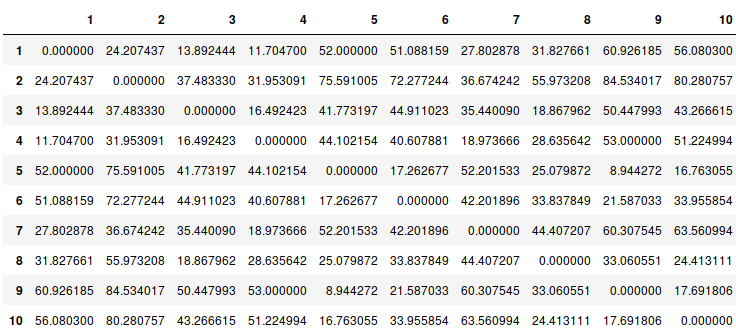
\includegraphics[width=\textwidth]{images/table.png}
\caption{Kimenet}
\label{fig:kimenet}
\end{figure}

Inicializáljuk a pointCount értékét 10-re, ennyi helyre kell a futárnak eljutnia.

\begin{python}
pointCount = 10
\end{python}

A travel egy adott számból álló lista (jelen esetben 10 számból áll), amely a pontok meglátogatására utal. Feltételezzük, hogy zárt hurokra van szükség, így az utolsó pont autómatikusan csatlakozik az elsőhöz.


\begin{python}
travel = random.sample(range(pointCount), pointCount);}
\end{python}

Elindítunk egy ciklust az adott értékekkel


\begin{python}
for tlp in numpy.logspace(0, 5, num = 100000)[::-1]:
\end{python}


Két pont véletlenszerű cseréjével új új utat képzünk. Úgy valósítom meg, hogy választok két számot az i-t és a j-t. Összeállítom a newTravel-t a régi travel másolásával az i indexig, majd összefűzöm a j-edik travelel-t és egészen folytatom addig, amíg a j nem éri el az i-edik pontot, majd befejezem a travel többi részét.


\begin{python}
[i, j] = sorted(random.sample(range(pointCount), 2));
newTravel = travel[:i] + 
			travel[j:j + 1] + 
			travel[i + 1:j] + 
			travel[i:i + 1] + 
			travel[j + 1:]
\end{python}


Ha az if értéke igaz akkor a travel megkapja a newTravel értékét, az előzöekben említett csere miatt ez már változott. Az elképzelés az, hogy minimalizálni szeretnénk a pontok közti távolságok költségének összegét. Ehhez a Gibb-s faktor-t használtam fel, aminek lényege, az új állapotba való átmenet valószínűsége. Csak az i-edik és j-edik pontok közötti távolságokat szükséges összegezni, mivel a többi távolság ugyanaz mint a travel-ben mint a newTravel-ben egyaránt. Ha a faktor > 1 akkor az új költség alacsonyabb, travel megkapja a newTravel értékét.


\begin{python}
traveld = sum([
	math.sqrt(
		sum([(
			(
			  (points[travel[(k + 1) % pointCount]][d]) - 
			  (points[travel[k % pointCount]][d])
			) **  2
		) for d in [0, 1]])
	) for k in [j, j - 1, i, i - 1]
])
newTraveld = sum([
	math.sqrt(
		sum([(
			(
			  (points[newTravel[(k + 1) % pointCount]][d]) - 
			  (points[newTravel[k % pointCount]][d])) 
			** 2
		) for d in [0, 1]])
	) for k in [j, j - 1, i, i - 1]
])
    if math.exp((traveld - newTraveld) / tlp) > random.random():
        travel = copy.copy(newTravel);
\end{python}        


Az algoritmus végeztével már csak meg kell jeleníteni a kívánt pontokat, ez kirajzol egy gráfot, amely optimális utat ad. Ehhez a pyplot libary-t használtam


\begin{python}
plt.plot(
	[points[
		travel[i % pointCount]][0] for i in range(pointCount + 1)
	], 
	[points[
		travel[i % pointCount]][1] for i in range(pointCount + 1)
	], 
	'xb-'
)
plt.show()
\end{python}

Kapcsolódó problémák

Adott teljes élsúlyozott gráf esetén keressük a legkisebb összsúllyal rendelkező Hamilton-kört. Megmutatható, hogy a kiindulási városba való visszatérés megkövetelése nem nehezít a probléma számítási nehézségén, tehát minimális súlyú Hamilton-út keresése egy adott pontból is NP-teljes.
A probléma egy másik változata, amikor nem a legkisebb súlyú Hamilton-kört keressük, hanem azt, amelyikben a „legnehezebb” él súlya a lehető legkisebb. A logisztikai problémákon túl nagy gyakorlati jelentőséggel bír például a nyomtatott áramkörök gyártása során fúrórobotok ideális mozgásának megtervezésében.

\Section{Több étterem, egy futár, több kiszállítás esete}

\Section{Egy étterem, több futár, több kiszállítás esete}

\Section{Több étterem, több futár, több kiszállítás esete}
